\chapter{Background}
\section{Machine Learning}
    Machine learning (ML) is a branch of artificial intelligence that focuses on creating models and algorithms that allow computers to learn from data and make decisions or predictions without needing to be explicitly programmed. ML is based on learning from examples or experience, in which computers repeatedly identify relationships in datasets to improve their performance on a particular task. The concepts of training and inference are fundamental to ML. In training, an algorithm learns from data by modifying its internal parameters. In inference, a trained model uses its newly acquired knowledge to predict or make decisions based on new, unseen data. ML includes several subfields, such as reinforcement learning, unsupervised learning, and supervised learning, each suitable for a distinct learning scenario. All things considered, ML is essential for solving complex problems in a variety of fields, including speech and picture recognition, natural language processing, and autonomous systems.\clearpage
    %##########################################################
    \subsection{Supervised Learning}
    A key machine learning concept is supervised learning, in which algorithms pick up predictions or decisions through labeled data. Pairs of inputs and outputs, each of which is connected to a target label or equivalent output, make up the training data for supervised learning. Finding a mapping from inputs to outputs that works effectively for unknown data is the primary objective of supervised learning as shown in Fig. \ref{fig:SL}. The algorithm modifies its internal parameters during training to reduce the error between the true labels in the training data and its predictions. Classification and regression are two common supervised learning tasks in which the algorithm predicts discrete class labels for input data and continuous numeric values, respectively. Wide-ranging applications of supervised learning can be found in fields like medical diagnosis, natural language processing, and picture identification, where labeled data is easily accessible for training prediction models.
        \begin{figure}[H]
            \centering
            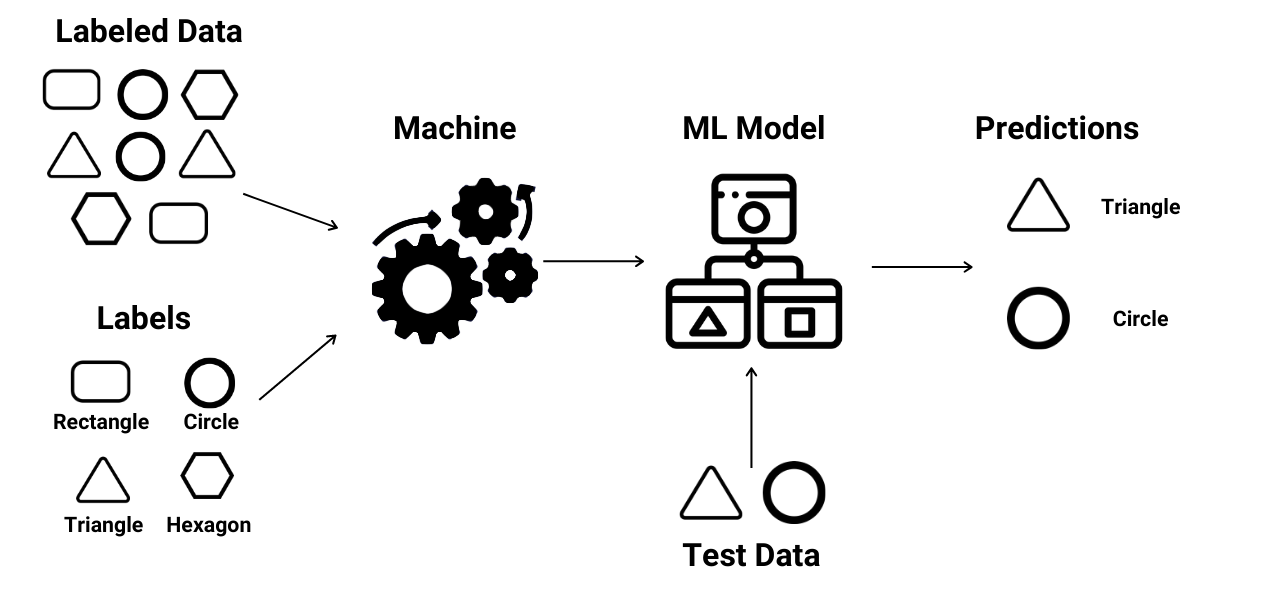
\includegraphics[width=0.9\linewidth]{Images/supervised.png}
            \caption{Supervised Machine Learning Illustration \cite{Raj_2022}}
            \label{fig:SL}
        \end{figure}\clearpage
        %#####################################################
    \subsection{Unsupervised Learning}
   In the field of unsupervised learning, computers identify patterns and structures from unlabeled data without the need for direct supervision or instructions. Unsupervised learning techniques investigate the basic structure of the data to find hidden patterns or relationships, as shown in Fig. \ref{fig:USL}, in contrast to supervised learning, which trains the algorithm using labeled examples.
   \begin{figure}[H]
            \centering
            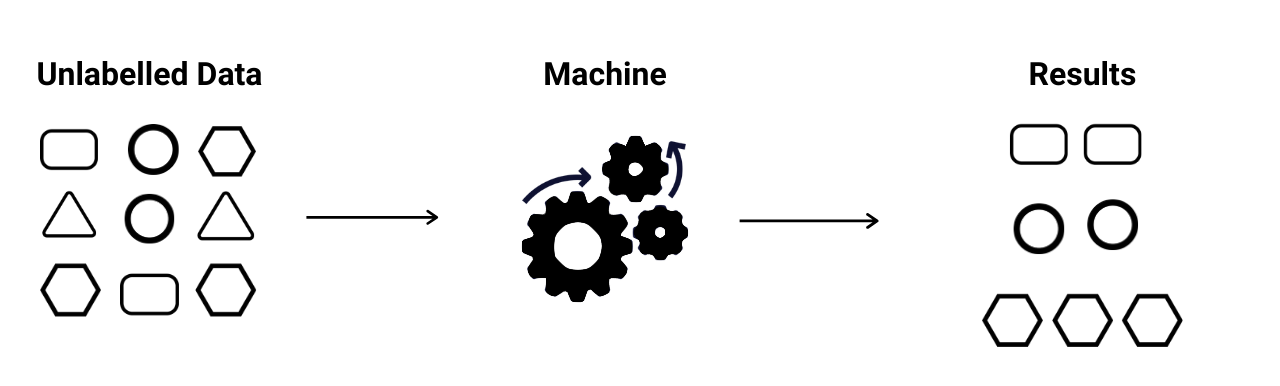
\includegraphics[width=0.9\linewidth]{Images/unsupervised.png}
            \caption{Unsupervised Machine Learning Illustration \cite{Raj_2022}}
            \label{fig:USL}
    \end{figure}
   Under unsupervised learning, common objectives include dimensionality reduction, reducing the number of features in the data while maintaining the important information, and clustering, the process by which an algorithm puts together similar data points. To extract valuable insights from unprocessed data, unsupervised learning algorithms use methods including principal component analysis (PCA), hierarchical clustering, and k-means clustering. Unsupervised learning has applications in a wide range of fields, such as data compression, anomaly detection, and data exploration, where it may be difficult or impossible to obtain labeled data.\clearpage
   %#########################################################
   \subsection{Reinforcement Learning}
        RL is a dynamic framework in machine learning that is characterized by its ability to provide agents with the opportunity to independently learn the best ways to make decisions by interacting with their environment. Compared to conventional supervised learning, it is a fundamentally different approach because RL agents live in an environment where they actively explore and interact with their surroundings rather than relying on pre-labeled data. A continuous feedback loop is at the core of the learning process. RL agents take actions in their environment, get feedback in the form of rewards or penalties depending on how their actions turn out as shown in Fig. \ref{fig:RL}, and then modify their behavior to maximize the rewards over the long run.
        \begin{figure}[H]
            \centering
            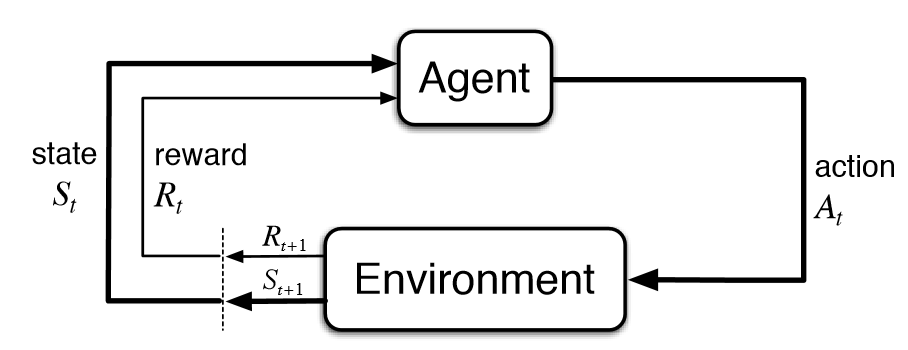
\includegraphics[width=0.9\linewidth]{Images/RL.png}
            \caption{Reinforcement Learning Framework Block Diagram \cite{RL}}
            \label{fig:RL}
    \end{figure}
        Using this iterative process of trial and error learning, RL agents can adapt to uncertainty, navigate complex environments, and gradually improve their decision-making techniques over time. The core concept of RL is made up of fundamental concepts such as states, actions, rewards, and policies. These concepts offer a framework for agents to learn and improve their behavior. Robotics, finance, healthcare, and other areas are all being revolutionized by RL, which gives systems the ability to learn and act independently in complex and uncertain environments.\clearpage
    %###############################################################
    \subsection{Neural Networks}
    Inspired by the architecture of the human brain, neural networks are extremely strong computer models that can extract complicated patterns from data. These networks, which consist of interconnected layers of neurons, are particularly good at tasks like speech recognition, picture recognition, and natural language processing. Neural networks can extract useful information from unprocessed data and improve their predictive power through the adjustment of internal parameters during training.
    \begin{figure}[H]
            \centering
            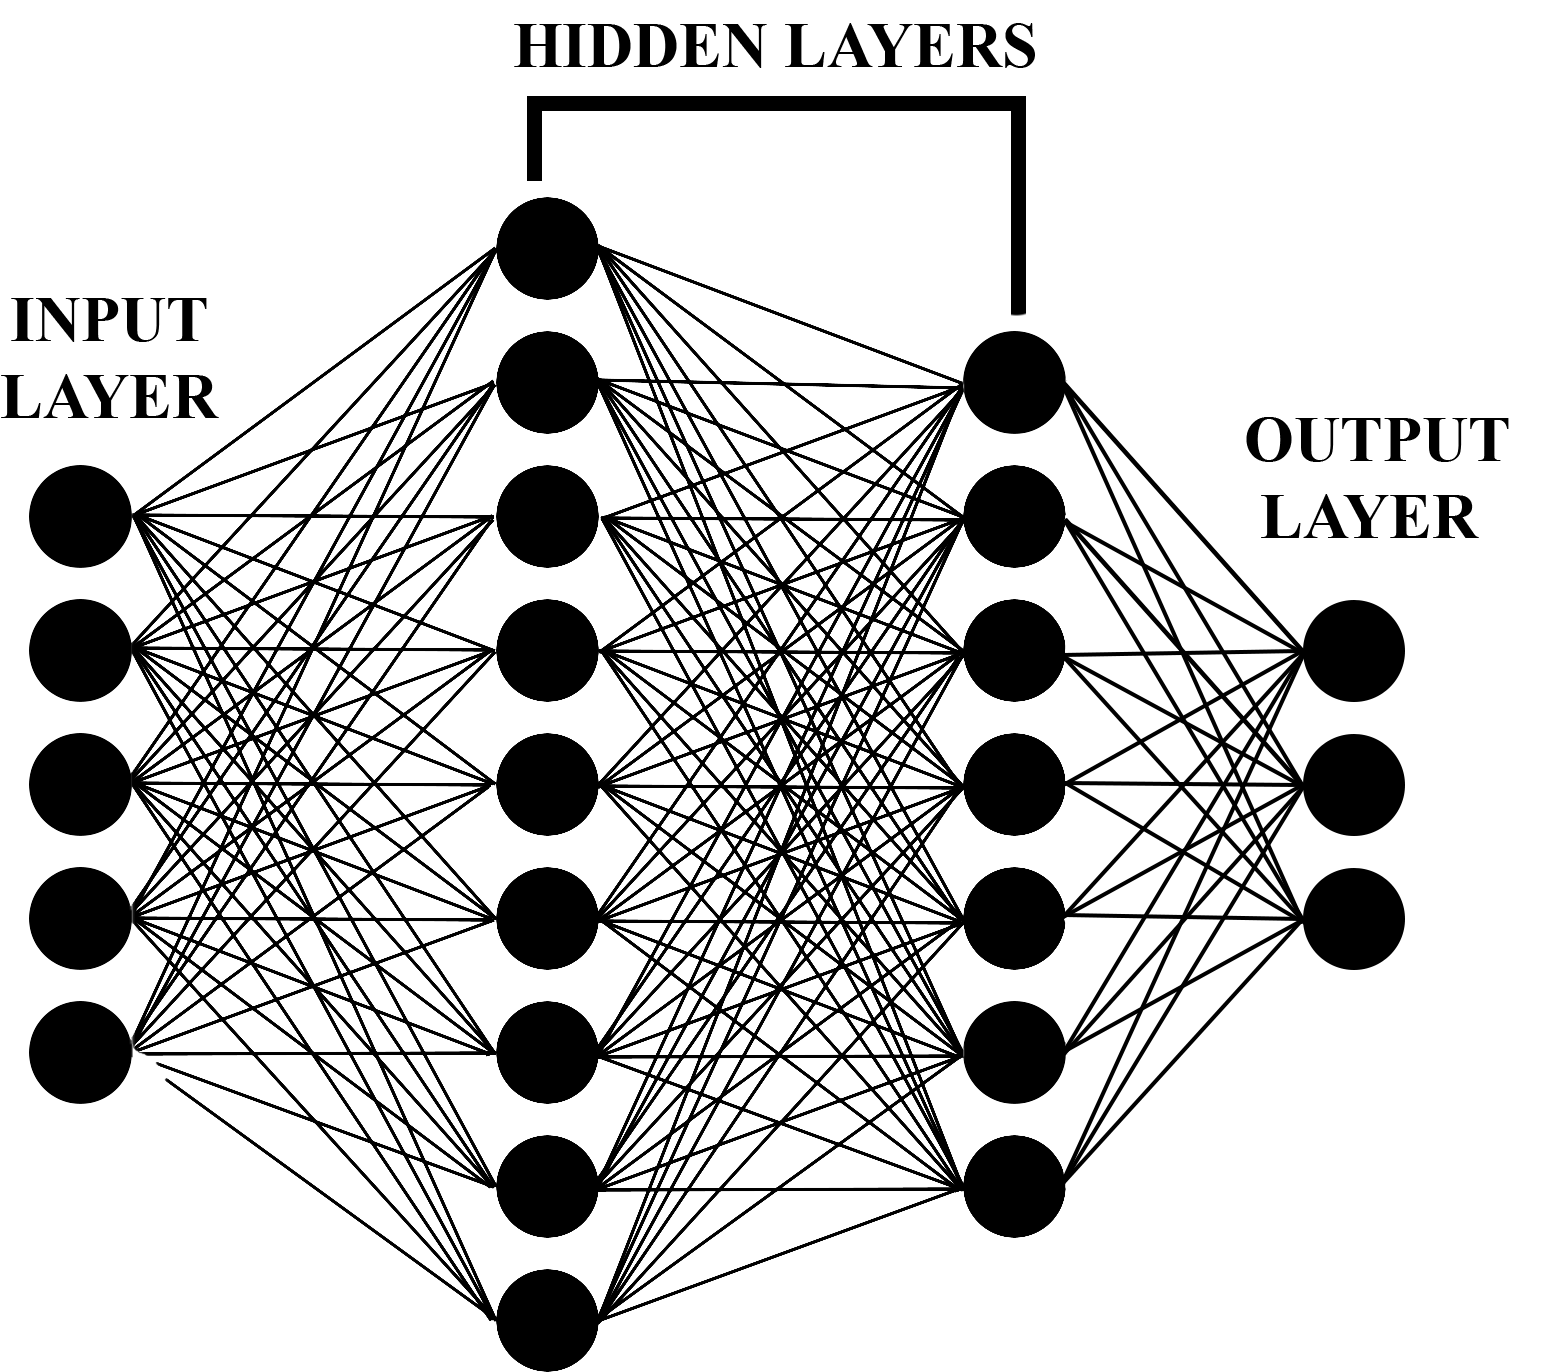
\includegraphics[width=0.6\linewidth]{Images/actor.png}
            \caption{Neural Network Structure}
            \label{fig:NN}
    \end{figure}
    A key factor in determining how neural networks function is the complex relationship between layers and weights. Input, hidden, and output layers are all interconnected as showin in Fig. \ref{fig:NN} and perform different functions related to data processing in these networks. Weights, which represent the strength of interconnections between neurons, are used by the neurons nested inside these layers to communicate with one another. In the training phase, these weights are iteratively adjusted through the use of backpropagation, a complex method that carefully propagates errors backward through the network. This makes it possible to fine-tune to reduce the error between expected and actual outcomes. Moreover, important non-linearity is introduced into the network's computations by activation functions like sigmoid, ReLU (Rectified Linear Unit), and tanh (hyperbolic tangent), which allow the network to identify complex patterns and relationships in the data. Each layer in the network applies the activation function to the weighted sum of inputs as data flows through it during the forward pass, turning raw data into increasingly abstract representations. Neural networks can extract subtle elements from the data through this iterative process, which gives them the ability to perform exceptionally well in tasks such as image recognition, natural language processing, and predictive analytics. Backpropagation effectively modifies the network's parameters to maximize its performance using sophisticated mathematical functions and algorithms, such as derivatives and gradients. This process promotes the development of progressively more complex and precise predictive models.
    %###########################################################
    \subsection{Deep RL}
    As a combination of deep neural network designs and RL concepts, deep RL is the peak of modern artificial intelligence. In this framework, agents use deep learning to extract complex patterns and representations from raw sensory inputs in addition to learning optimal decision-making procedures. When RL and deep neural networks are combined, agents can function in high-dimensional, complex environments like video games, robotics, and autonomous quadcopters with maximum efficiency. Deep neural networks are used by agents in deep RL to approximate value functions or policies that dictates decision-making as they navigate a large space of states and actions. Furthermore, deep RL algorithms, like TD3, SAC, and Deep Deterministic Policy Gradient (DDPG), have proven to be remarkably effective at a variety of difficult tasks, including superhuman performance in robotic control and navigation and the ability to master complex video games. Deep RL marks a new era of intelligent systems that are capable of autonomous learning and adaptation in dynamic and uncertain environments. This is made possible by the collaboration of RL principles and deep neural network architectures, and it will open the door for revolutionary advancements in a variety of scientific and technological fields.
    %#############################################################3
    \subsection{DDPG Algorithm}
    The TD3 algorithm is a continuation of the DDPG algorithm. To understand the key concepts of TD3, DDPG must be explored first. The DDPG consists of an actor network, a target actor network, a critic network, and a target critic network.
    The DDPG algorithm and all the proposed equations are based on the DDPG original implementation \cite{silver2014deterministic} \cite{lillicrap2019continuous}. DDPG is an off-policy algorithm that learns a Q-function through the Bellman equation and a policy through the Q-function. \\
    
    Similar to the Q-learning, if you know the optimal action value function $Q^*(s, a)$, then the optimal action $a^*(s)$ can be found through Eq. \ref{eq1}.\\
    \begin{equation}
    a^*(s) = \hspace{5pt}\substack{\mathlarger{\text{argmax}} \\ \mathlarger{a}}\hspace{3pt} Q^*(s,a)
        \label{eq1}
    \end{equation}
    \begin{enumerate}[label={\alph*)}]
        \item Q-Learning in DDPG\\
        The Bellman equation describing the action-value function $Q^*(s,a)$ is shown in Eq. \ref{eq2}.\\
        \begin{equation}
    Q^*(s,a) = \substack{\mathlarger{\text{E}} \\ s' \thicksim P}\hspace{5pt} [r(s,a) + \gamma\hspace{5pt} \substack{\mathlarger{\text{max}} \\ \mathlarger{a'}}\hspace{5pt} Q^*(s',a')] 
        \label{eq2}
    \end{equation}\\
    where $s'$ is sampled by the environment from a distribution $P(.|s,a)$.
    Eq. \ref{eq2} is the initial point to learn an approximator to $Q^*(s,a)$. Suppose the approximator is a neural network $Q_{\phi}(s, a)$, with parameters $\phi$, and a batch is collected from buffer $D$. Using the Mean Squared Bellman Error (MSBE) function the loss function is shown in Eq. \ref{eq3}.\\
    \begin{equation}
    L(\phi, D) = \substack{\mathlarger{\mathlarger{\text{E}}} \\ (s, a,r,s',d) \thicksim D}\hspace{5pt} \Bigg[\bigg(Q_{\phi}(s, a) - \Big(\gamma (1-d) \hspace{5pt} \substack{\mathlarger{\text{max}} \\ \mathlarger{a'}}\hspace{5pt} Q_{\phi}(s', a')\Big)\bigg)^2\Bigg] 
        \label{eq3}
    \end{equation}
    Q-learning makes use of an experience replay buffer $D$. A large enough replay buffer ensures a stable behavior. Too large buffers cause over-fitting problems and produce unstable behavior. So, a suitable buffer size must be chosen.\\
    Q-learning also makes use of target networks defined by Eq. \ref{eq4}.
    \begin{equation}
    r + \gamma (1 - d) \hspace{5pt} \substack{\mathlarger{\text{max}} \\ \mathlarger{a'}}\hspace{5pt} Q_{\phi}(s',a')
        \label{eq4}
    \end{equation}
    When minimizing the MSBE the Q-functions tend to equal the value of Eq. \ref{eq4}. To ensure stable behavior a target network is used with a set of parameters $\phi_{targ}$  which lags the original parameters $\phi$ of the Q-function. The target network is updated using Polyak averaging once per main network update as shown in Eq. \ref{eq5}.\\
    \begin{equation}
    \phi_{targ} \leftarrow \rho \phi_{targ} + (1 - \rho)\phi \hspace{15pt} where \hspace{5pt}\rho \in [0,1]
        \label{eq5}
    \end{equation}\\
    To calculate the maximum over actions, DDPG uses a target policy network to compute an action that maximizes $Q_{\phi_{targ}}$. The target policy parameters are found using Polyak averaging as shown in Eq. \ref{eq5}.\\

    The final loss function to be minimized is presented by Eq. \ref{eq6} where $\mu_{\vartheta_{targ}}(s')$ is the target policy.\\
    \begin{equation}
    L(\phi, D) = \substack{ \mathlarger{\mathlarger{\text{E}}}  \\ (s,a,r,s',d) \thicksim D}\hspace{5pt} \Bigg[\bigg(Q_{\phi}(s, a) - \Big(r + \gamma (1-d)  Q_{\phi_{targ}}(s',\mu_{\vartheta_{targ}}(s'))\Big)\bigg)^2\Bigg]  
        \label{eq6}
    \end{equation}
    \item Policy Learning in DDPG\\
    A deterministic policy $\mu_{\vartheta}(S)$ is learnt where it maximizes $Q_{\phi}(s,a)$. The Q-function is differentiable with respect to action due to the continuous nature of the action space. A gradient ascent is used to solve Eq. \ref{eq7}.
    \begin{equation}
    \substack{\mathlarger{\text{max}} \\ \mathlarger{\vartheta}} \hspace{5pt} \substack{\mathlarger{\text{E}} \\ s \thicksim D} \hspace{5pt} [Q_{\phi}(s, \mu_{\vartheta}(s))]  
        \label{eq7}
    \end{equation}\clearpage
    \item Exploration\\
    Exploration is done off-policy in DDPG. Action noise is added to the output action at training time.
    \end{enumerate}
    A brief explanation of the DDPG is presented as a pseudocode in Table \ref{DDPG}.
    
         \begin{table}[H]
   \centering
   \begin{tabular}{l}
   \hline
    \textbf{Algorithm 1} Deep Deterministic Policy Gradient \\
    \hline
    \setstretch{0.05}\\
    \begin{minipage}{0.9\linewidth}
    \setstretch{1}
        \begin{enumerate}[label={\arabic*:}]
            \item Input: initial policy parameters $\vartheta$, Q-function parameters $\phi$, empty replay buffer $D$
            \item Set target parameters equal to main parameters $\vartheta_{targ}$ $\leftarrow$ $\vartheta$, $\phi_{targ}$ $\leftarrow$ $\phi$
            \item \textbf{repeat}
            \item \hspace{10pt} Observe state $s$ and select action $a = clip(\mu_{\vartheta}(s) + \epsilon, a_{Low}, a_{High})$, where $\epsilon \thicksim N$
            \item \hspace{10pt} Execute $a$ in the environment
            \item \hspace{10pt} Observe next state $s'$, reward $r$, and done signal $d$ to indicate whether $s'$ is terminal
            \item \hspace{10pt} Store ($s, a, r, s', d$) in replay buffer $D$
            \item \hspace{10pt} if $s'$ is terminal, reset environment state
            \item \hspace{10pt} \textbf{if} it's time to update \textbf{then}
            \item \hspace{20pt} \textbf{for} $j$ in range (how many updates) \textbf{do}
            \item \hspace{30pt} Randomly sample a batch of transitions, $B = {(s, a, r, s', d)}$ from $D$
            \item \hspace{30pt} Compute targets\\
                \centerline{$y(r, s', d) = r + \gamma(1-d)\text{  } Q_{\phi_{targ}} (s', \mu_{\vartheta_{targ}}(s'))$}
            \item \hspace{30pt} Update Q-functions by one step of gradient descent using\\
                \centerline{$\nabla_{\phi} \text{  } \frac{1}{|B|} \text{  } \substack{\displaystyle\sum \\ (s,a,r,s',d) \in B} \text{  } (Q_{\phi} (s,a) - y(r,s',d))^2$ }
            \item \hspace{40pt} Update policy by one step of gradient ascent using\\
                \centerline{$\nabla_{\vartheta} \text{  } \frac{1}{|B|} \text{  } \substack{\displaystyle\sum \\ s \in B} \text{  } Q_{\phi} (s, \mu_{\vartheta}(s))$}
            \item \hspace{40pt} Update target networks with\\
                \centerline{$\phi_{targ} \leftarrow \rho \text{ } \phi_{targ} + (1-\rho) \phi$}\\
                \centerline{$\vartheta_{targ} \leftarrow \rho \text{ } \vartheta_{targ} + (1 - \rho) \vartheta$}
            \item \hspace{20pt} \textbf{end for}
            \item \hspace{10pt} \textbf{end if}
            \item \textbf{until} convergence
        \end{enumerate}
    \end{minipage} \\
    \hline
    \end{tabular}
    \caption{Pseudocode of DDPG Algorithm \cite{lillicrap2019continuous}}
    \label{DDPG}
\end{table}\clearpage
    %#######################################################
    \subsection{TD3 Algorithm}
    The TD3 algorithm is a continuation of the DDPG algorithm. The TD3 algorithm solves the Q-value overestimation problem of the DDPG algorithm which leads to policy breaking. This is done using three methods.
    \begin{enumerate}
        \item \textbf{Clipped Double Q-learning "Twin":} this is done by learning two Q-functions and using the minimum Q-value to create the targets using Bellman's Equation
        \item \textbf{"Delayed" Policy Updates:} The TD3 does one policy update every two Q-function updates
        \item \textbf{Target Policy Smoothing:} By adding noise to the target action, it is harder to exploit Q-function errors by smoothing out Q-values along the action.
    \end{enumerate}
    Fig. \ref{TD3 Block Diagram} shows a block diagram schematic for the TD3 algorithm explained in this section. The TD3 consists of an actor network, a target actor network, 2 critic networks, and 2 target critic networks.
    \begin{figure}[H]
            \centering
            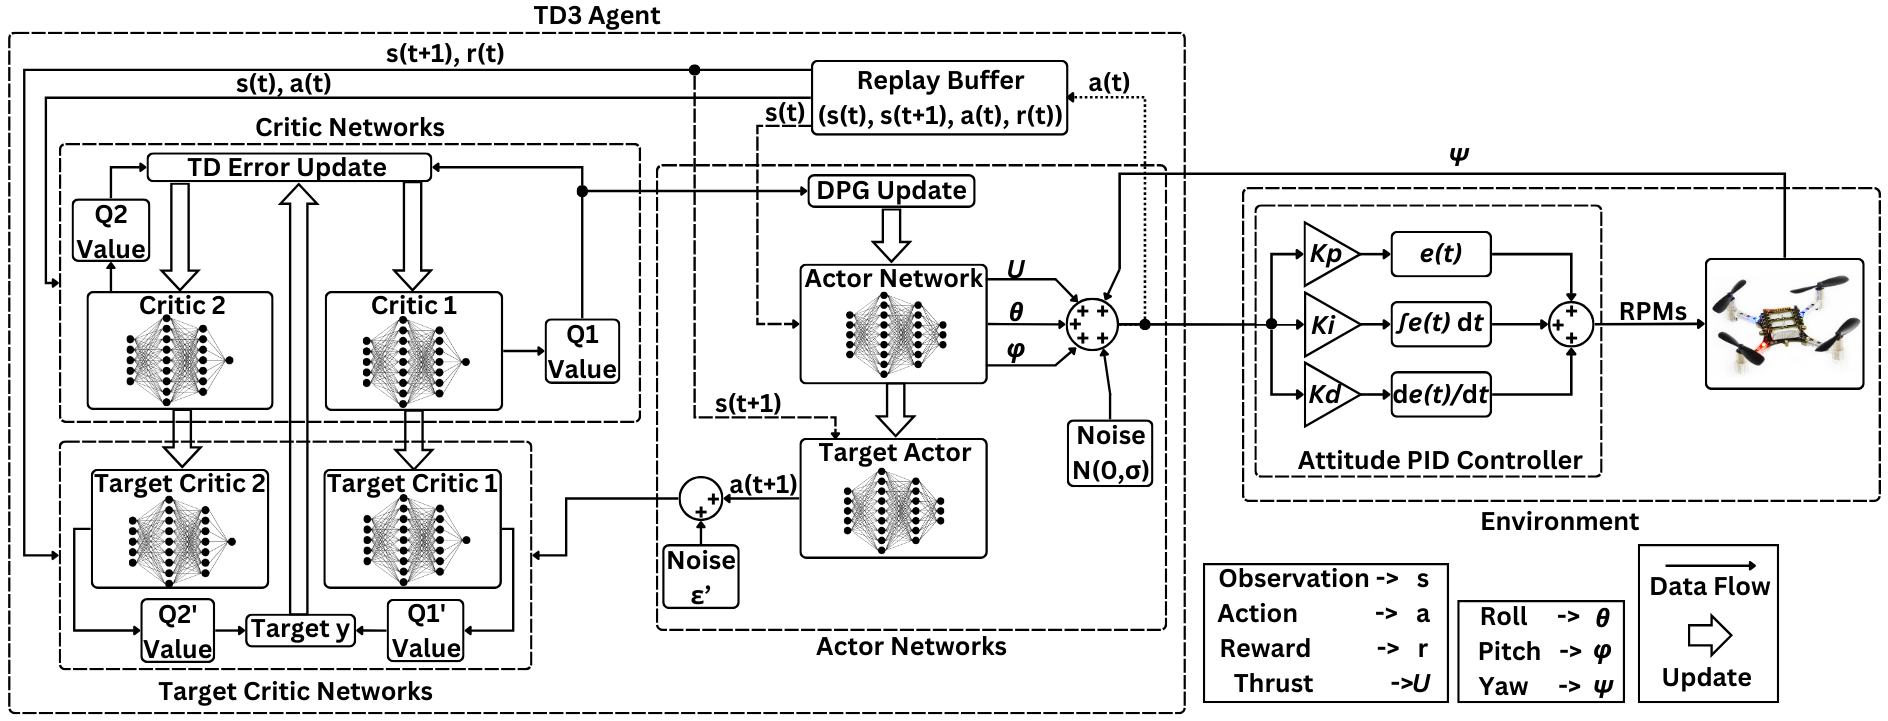
\includegraphics[width=1\linewidth]{Images/TD3.png}
            \caption{Block Diagram of Used TD3 Position Controller Agent}
            \label{TD3 Block Diagram}
    \end{figure}
    The TD3 algorithm and all the proposed equations are based on the TD3 original implementation \cite{fujimoto2018addressing}. TD3 learns two Q-functions in almost the same way DDPG learns its Q-function and estimates a deterministic policy. 
    \clearpage
    The changes done to the Q-function learning is shown as follows:
    \begin{enumerate}[label={\alph*)}]
        \item Target Policy Smoothing\\
        The actions used to update the target critic networks are based on the target policy $\mu_{\vartheta_{targ}}$ with clipped noise added to it. The action is then clipped to ensure it stays in the action range. The action is computed using Eq. \ref{eq8}
        \begin{equation}
            a'(s') = clip (\mu_{\vartheta_{targ}}(s') + clip (\epsilon, -c, c), a_{Low}, a_{High}), \hspace{15pt} \epsilon \thicksim N(0,\sigma)  
        \label{eq8}
    \end{equation}
    \item Clipped Double Q-Learning\\
    The single target value is calculated using Eq. \ref{eq9}.
    \begin{equation}
        y(r, s', d) = r + \gamma (1 - d) \hspace{5pt} \substack{\mathlarger{\text{min}} \\ i = 1,2} \hspace{5pt} Q_{\phi_{i,targ}}(s',a'(s')) 
        \label{eq9}
    \end{equation}
    The Loss function parameterizing the Q-functions is shown in Eq. \ref{eq10} and Eq. \ref{eq11}.
    \begin{equation}
        L(\phi_{1}, D) = \substack{ \mathlarger{\mathlarger{\text{E}}}  \\ (s,a,r,s',d) \thicksim D}\hspace{5pt} \bigg[\Big(Q_{\phi_{1}}(s, a) - y(r, s', d) \Big)^2 \bigg]
        \label{eq10}
    \end{equation}
    \begin{equation}
        L(\phi_{2}, D) = \substack{ \mathlarger{\mathlarger{\text{E}}}  \\ (s,a,r,s',d) \thicksim D}\hspace{5pt} \bigg[\Big(Q_{\phi_{2}}(s, a) - y(r, s', d) \Big)^2 \bigg]
        \label{eq11}
    \end{equation}
    \item Policy Learning\\
    Same as the DDPG algorithm, the policy is learned by maximizing $Q_{\phi_{1}}$ as shown in Eq. \ref{eq12}.
    \begin{equation}
        \substack{\mathlarger{\text{max}} \\ \mathlarger{\vartheta}} \hspace{5pt} \substack{\mathlarger{\text{E}} \\ s \thicksim D} \hspace{5pt} [Q_{\phi_{1}}(s, \mu_{\vartheta}(s))] 
        \label{eq12}
    \end{equation}
    \end{enumerate}
    A brief pseudocode of the TD3 algorithm used in training is shown in Table \ref{TD3}.
        \begin{table}[H]
   \centering
   \begin{tabular}{l}
   \hline
    \textbf{Algorithm 2} Twin Delayed DDPG \\
    \hline
    \setstretch{0.05}\\
    \begin{minipage}{0.9\linewidth}
    \setstretch{1}
        \begin{enumerate}[label={\arabic*:}]
            \item Input: initial policy parameters $\vartheta$, Q-function parameters $\phi_{1}$, $\phi_{2}$, empty replay buffer $D$ of size $2 \times 10^6$
            \item Set target parameters equal to main parameters $\vartheta_{targ}$ $\leftarrow$ $\vartheta$, $\phi_{targ,1}$ $\leftarrow$ $\phi_{1}$, $\phi_{targ,2}$ $\leftarrow$ $\phi_{2}$
            \item \textbf{repeat}
            \item \hspace{10pt} Observe state s = $[\theta, \varphi,\psi, v_{x}, v_{y}, v{z}, w_{\theta}, w{\varphi}, w_{\psi}, \Delta x,\Delta y, \Delta z]$ and select action \\ \color{white} y \color{black}\hspace{5pt}$a = clip(\mu_{\vartheta}(s) + \epsilon, -1, 1)$, where $\epsilon \thicksim N$ and $\mu_{\vartheta}(s) = (U_{1}, \theta, \varphi)$
            \item \hspace{10pt} Send $a$ to the PID attitude controller
            \item \hspace{10pt} Execute PID attitude controller action in environment
            \item \hspace{10pt} reward $r = \frac{1}{a \text{  }* \text{  }||\vec{e}_{k}||_{2}} + \frac{a}{\sqrt{2\pi \sigma^2}} e^{-0.5(\frac{||\vec{e}_{k}||_{2}}{\sigma})^2}$
            \item \hspace{10pt} done signal $d = true$ when episode length = 502 steps or $x < -2.9$ or  $x > 2.9$ or\\ \color{white} y \color{black}\hspace{5pt}$y < -2.9$ or $y > 2.9$ or $z < 0.1$ or $z > 2.9$
            \item \hspace{10pt} Observe next state $s'$, reward $r$, and done signal $d$ to indicate whether $s'$ is terminal
            \item \hspace{10pt} Store ($s, a, r, s', d$) in replay buffer $D$
            \item \hspace{10pt} if $s'$ is terminal, reset environment state
            \item \hspace{10pt} \textbf{if} it's time to update \textbf{then}
            \item \hspace{20pt} \textbf{for} $j$ in range (6e6) \textbf{do}
            \item \hspace{30pt} Randomly sample a batch of transitions, $B = {(s, a, r, s', d)}$ from $D$
            \item \hspace{30pt} Compute Target Actions\\
                \centerline{$a'(s')= clip(\mu_{\vartheta_{targ}}(s') + clip(\epsilon, -c,c), -1, 1) \hspace{20pt} \epsilon \thicksim N(0, \sigma)$}
            \item \hspace{30pt} Compute targets\\
                \centerline{$y(r, s', d) = r + \gamma(1-d)\text{  } \substack{\min \\ i=1,2} \text{  } Q_{\phi_{targ,i}} (s', a'(s'))$}
            \item \hspace{30pt} Update Q-functions by one step of gradient descent using\\
                \centerline{$\nabla_{\phi_{i}} \text{  } \frac{1}{|B|} \text{  } \substack{\displaystyle\sum \\ (s,a,r,s',d) \in B} \text{  } (Q_{\phi_{i}} (s,a) - y(r,s',d))^2$ \hspace{20pt} for $i = 1,2$}
            \item \hspace{30pt} \textbf{if} $j \mod$ policy\_delay = 0 \textbf{then}
            \item \hspace{40pt} Update policy by one step of gradient ascent using\\
                \centerline{$\nabla_{\vartheta} \text{  } \frac{1}{|B|} \text{  } \substack{\displaystyle\sum \\ s \in B} \text{  } Q_{\phi_{1}} (s, \mu_{\vartheta}(s))$}
            \item \hspace{40pt} Update target networks with\\
                \centerline{$\phi_{targ,i} \leftarrow \rho \text{ } \phi_{targ,i} + (1-\rho) \phi_{i}$  for $i = 1,2$}\\
                \centerline{$\vartheta_{targ} \leftarrow \rho \text{ } \vartheta_{targ} + (1 - \rho) \vartheta$}
            \item \hspace{30pt} \textbf{end if}
            \item \hspace{20pt} \textbf{end for}
            \item \hspace{10pt} \textbf{end if}
            \item \textbf{until} convergence
        \end{enumerate}
    \end{minipage} \\
    \hline
    \end{tabular}
    \caption{Pseudocode of Used TD3 Position Controller Agent \cite{fujimoto2018addressing}}
    \label{TD3}
\end{table}
    %#######################################################################
    \subsection{SAC Algorithm}
    The SAC algorithm trains a stochastic policy using off-policy methods. Inheriting the clipped double Q-learning, the SAC is similar to the TD3 algorithm. The main feature of the SAC algorithm is entropy regularization which maximizes a trade-off between rewards and entropy, the randomness in the policy. Fig. \ref{SAC Block Diagram} shows a block diagram schematic for the SAC algorithm explained in this section. The SAC consists of an actor network, 2 critic networks, and 2 target critic networks.
    \begin{figure}[H]
            \centering
            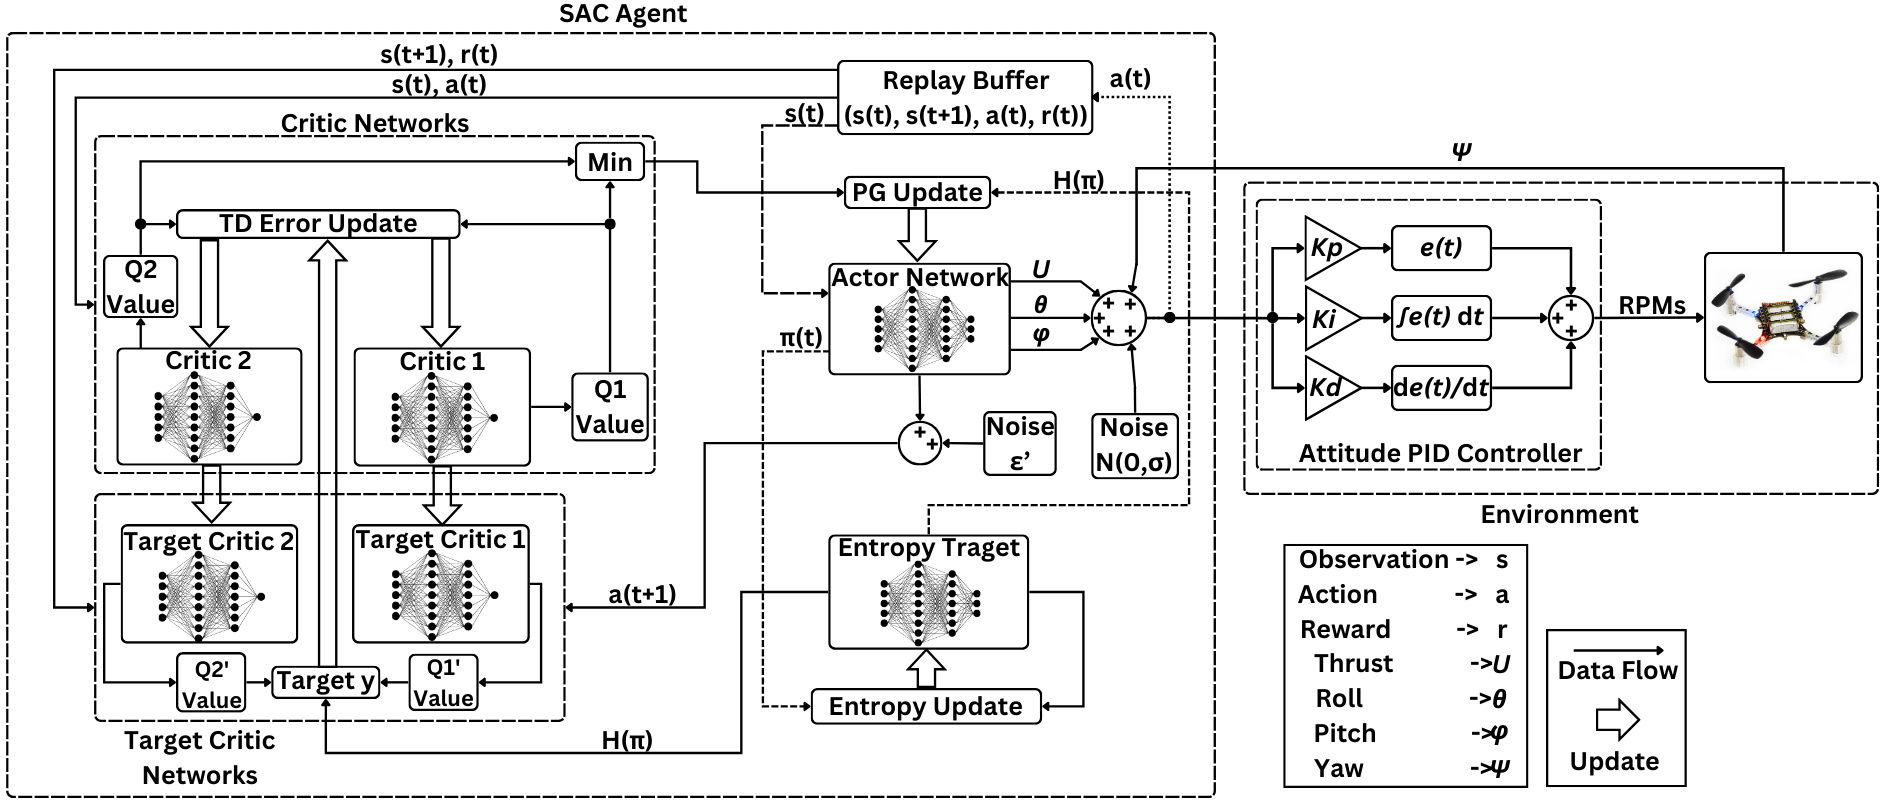
\includegraphics[width=1\linewidth]{Images/SAC.png}
            \caption{Block Diagram of Used SAC Position Controller Agent}
            \label{SAC Block Diagram}
    \end{figure}
    The SAC algorithm and all the proposed equations are based on the SAC original implementation \cite{haarnoja2019soft} \cite{haarnoja2018soft} \cite{haarnoja2019learning}.
    \begin{enumerate}[label={\alph*)}]
        \item Entropy Regularization\\
        Entropy is the measure of how random a variable is. Let $x$ be a random variable with probability density function $P$. The entropy $H$ of $x$ is computed as shown in Eq. \ref{eq13}.
        \begin{equation}
        H(P) = \substack{\mathlarger{\text{E}} \\ x \thicksim P} \hspace{5pt}[-\log P(x)]
        \label{eq13}
    \end{equation}
    The agent receives a bonus reward at each time step proportional to the entropy at that time step changing the optimal policy to Eq. \ref{eq14}.
    \begin{equation}
        \pi^* = \substack{\mathlarger{\text{argmax}} \\ \mathlarger{\pi}} \hspace{2pt} \substack{\mathlarger{\text{E}} \\ \tau \thicksim \pi} \bigg[\sum_{t=0}^{\infty} \gamma^t \Big(R(s_{t}, a_{t}, s_{t+1}) + \alpha H (\pi(.|s_{t})) \Big)\bigg] \hspace{15pt} where \hspace{5pt} \alpha > 0
        \label{eq14}
    \end{equation}
    The value function $V^\pi$ is changed to Eq. \ref{eq15}.
    \begin{equation}
        V^\pi(s) = \substack{\mathlarger{\text{E}} \\ \tau \thicksim \pi} \bigg[\sum_{t=0}^{\infty} \gamma^t \Big(R(s_{t}, a_{t}, s_{t+1}) + \alpha H (\pi(.|s_{t})) \Big) \bigg| s_{0} = s \bigg]
        \label{eq15}
    \end{equation}
    $Q^\pi$ is changed to Eq. \ref{eq16}.
    \begin{equation}
        Q^\pi(s, a) = \substack{\mathlarger{\text{E}} \\ \tau \thicksim \pi} \bigg[\sum_{t=0}^{\infty} \gamma^t (R(s_{t}, a_{t}, s_{t+1}) + \alpha \sum_{t=1}^{\infty} \gamma^t H (\pi(.|s_{t})) ) \bigg| s_{0} = s, a_{0} = a \bigg]
        \label{eq16}
    \end{equation}
    $V^\pi$ and $Q^\pi$ are connected by Eq. \ref{eq17}.
    \begin{equation}
        V^\pi(s) = \substack{\mathlarger{\text{E}} \\ a \thicksim \pi}[Q^\pi(s,a)] + \alpha H (\pi(.|s))
        \label{eq17}
    \end{equation}
    The Bellman equation for $Q^\pi$ is Eq. \ref{eq18}.
    \begin{equation}
        Q^\pi(s, a) = \substack{\mathlarger{\text{E}} \\ s' \thicksim P\\ a' \thicksim \pi}[R(s, a, s') + \gamma (Q^\pi(s', a') + \alpha H (\pi(.|s')))]
        \label{eq18}
    \end{equation}
    \item Q-Learning\\
    SAC is similar to the TD3 as both Q-functions are minimized by regressing a single target, the shared target is computed using target critic networks, the target networks are obtained through Polyak averaging, and the shared target uses clipped double Q-learning.\\
    
    However, the SAC differs from the TD3 by adding an entropy term to the target, the next-state actions are computed from the current policy and no target policy smoothing is done as the SAC trains a stochastic policy and the stochastic noise is enough.\\

    Rewriting the $Q^\pi$ with the entropy definition gives Eq. \ref{eq19}.
    \begin{equation}
        Q^\pi(s, a) = \substack{\mathlarger{\text{E}} \\ s' \thicksim P\\ a' \thicksim \pi}[R(s, a, s') + \gamma (Q^\pi(s', a') - \alpha \log \pi(a'|s'))]
        \label{eq19}
    \end{equation}
    We can approximate it with samples giving Eq. \ref{eq20}.
    \begin{equation}
        Q^\pi(s, a) \approx r + \gamma (Q^\pi(s', \Tilde{a}') - \alpha \log\pi(\Tilde{a}'|s'))]\hspace{15pt} where \hspace{5pt} \Tilde{a}' \thicksim \pi(.|s')
        \label{eq20}
    \end{equation}
    The loss function is then given by Eq. \ref{eq21}.
    \begin{equation}
        L(\phi_{i}, D) = \substack{ \mathlarger{\mathlarger{\text{E}}}  \\ (s,a,r,s',d) \thicksim D}\hspace{5pt} \bigg[\Big(Q_{\phi_{i}} (s, a) - y(r, s', d) \Big)^2 \bigg]
        \label{eq21}
    \end{equation}
    With the target computed from Eq. \ref{eq22}.
    \begin{equation}
        y(r, s', d) = r + \gamma(1 - d) \bigg(\substack{\mathlarger{\text{min}} \\ j = 1,2}\hspace{5pt} Q_{\phi_{targ,j}}(s', \Tilde{a}') - \alpha \log \pi_{\vartheta}(\Tilde{a}' | s') \bigg) \hspace{15pt} where \hspace{5pt} \Tilde{a}' \thicksim \pi_{\vartheta}(.|s')
        \label{eq22}
    \end{equation}
    \item Policy Learning\\
    The policy is optimized using the reparameterization trick where a sample from $\pi_{\vartheta}(.|s)$ is drawn deterministically. The samples are obtained using a squashed Gaussian policy in Eq. \ref{eq23}.
    \begin{equation}
        \Tilde{a}_{\vartheta} (s, \zeta) = \tanh(\mu_{\vartheta}(s) + \sigma_{\vartheta}(s) \odot \zeta) \hspace{15pt} where \hspace{5pt} \zeta \thicksim N(0, I)
        \label{eq23}
    \end{equation}
    Rewriting the expectations over actions into expectations over noise in Eq. \ref{eq24}.
    \begin{equation}
        \substack{ \mathlarger{\mathlarger{\text{E}}}  \\ a \thicksim \pi_{\vartheta}}\hspace{5pt} [(Q^{\pi_{\vartheta}}(s, a) - \alpha \log \pi_{\vartheta}(a|s)] = \substack{ \mathlarger{\mathlarger{\text{E}}}  \\ \zeta \thicksim N}\hspace{5pt}[Q^{\pi_{\vartheta}}(s, \Tilde{a}_{\vartheta}(s, \zeta)) - \alpha \log \pi_{\vartheta} (\Tilde{a}_{\vartheta}(s, \zeta)|s)]
        \label{eq24}
    \end{equation}
    Getting the policy loss using Eq. \ref{eq25}.
    \begin{equation}
        \substack{\mathlarger{\text{max}} \\ \mathlarger{\vartheta}}\hspace{3pt} \substack{ \mathlarger{\mathlarger{\text{E}}}  \\ s \thicksim D \\ \zeta \thicksim N}\hspace{5pt} \Big[\substack{\mathlarger{\text{min}} \\ j=1,2}\hspace{5pt} Q_{\phi_{j}}(s, \Tilde{a}_{\vartheta}(s, \zeta)) - \alpha \log \pi_{\vartheta}(\Tilde{a}_{\vartheta}(s, \zeta)|s) \Big] 
        \label{eq25}
    \end{equation}\clearpage
    \item{Dynamic Entropy Tuning}\\
    Choosing the optimal entropy in entropy-based algorithm is a non-trivial task where the entropy is required to be tuned for each individual task \cite{haarnoja2019soft}. Dynamically tuning the entropy allows the policy to explore more in regions where the optimal policy is yet to be learned and to exploit more in areas where the optimal policy is already learned. This framework is crucial since the exploration-exploitation trade off is necessary for optimal policy learning. This framework also prevents catastrophic forgetting in deterministic RL algorithms where they tend to gradually worsen after reaching an optimal policy.\\
    
    We want to solve the constrained optimization problem presented in Eq. \ref{en1}.
    \begin{equation}
        \pi^* = \substack{\mathlarger{\text{argmax}} \\ \mathlarger{\pi}} \hspace{5pt}  \bigg[ \sum_{t} \substack{\mathlarger{\text{E}} \\(s_{t}, a_{t}) \thicksim \rho_{\pi_{\vartheta}}}\hspace{5pt} r(s_{t}, a_{t}) \bigg]\hspace{5pt} \text{s.t}\hspace{5pt} \forall t\hspace{3pt} \substack{\mathlarger{\text{E}} \\ (s_{t}, a_{t}) \thicksim \rho_{\pi_{\vartheta}}}\hspace{5pt} [-\log(\pi_{\vartheta}(a_{t}|s_{t}))]]\hspace{5pt} \geq\hspace{5pt } H_{0}
        \label{en1}
    \end{equation}
    Where $H_{0}$ is the desired minimum entropy.\\
    
    The final entropy loss function in Eq. \ref{en2} to be minimized is mathematically derived to fit the above mentioned constraint \cite{haarnoja2019soft}.
    \begin{equation}
        J(\alpha) = \substack{\mathlarger{\text{E}} \\ s_{t} \thicksim D}\hspace{5pt} \Big[\hspace{2pt}\substack{\mathlarger{\text{E}} \\ a_{t} \thicksim \pi_{\vartheta}(.|s_{t})}\hspace{5pt} [-\alpha \log \pi_{\vartheta} (a_{t}, s_{t}) - \alpha H_{0}] \Big]
        \label{en2}
    \end{equation}
    \end{enumerate}
A brief pseudocode of the SAC algorithm used in training is shown in Table \ref{SAC}.
    
            \begin{table}[H]
   \centering
   \begin{tabular}{l}
   \hline
    \textbf{Algorithm 3} Soft Actor-Critic \\
    \hline
    \setstretch{0.05}\\
    \begin{minipage}{0.9\linewidth}
    \setstretch{1}
        \begin{enumerate}[label={\arabic*:}]
            \item Input: initial policy parameters $\vartheta$, Q-function parameters $\phi_{1}$, $\phi_{2}$, empty replay buffer $D$ of size $2 \times 10^6$
            \item Set target parameters equal to main parameters $\phi_{targ,1}$ $\leftarrow$ $\phi_{1}$, $\phi_{targ,2}$ $\leftarrow$ $\phi_{2}$
            \item \textbf{repeat}
            \item \hspace{10pt} Observe state s = $[\theta, \varphi,\psi, v_{x}, v_{y}, v{z}, w_{\theta}, w{\varphi}, w_{\psi}, \Delta x,\Delta y, \Delta z]$ and select action \\ \color{white} y \color{black}\hspace{5pt}$a \thicksim \pi_{\vartheta} (.|s)$
            \item \hspace{10pt} Send $a$ to the PID attitude controller
            \item \hspace{10pt} Execute PID attitude controller action in environment
            \item \hspace{10pt} reward $r = \frac{1}{a \text{  }* \text{  }||\vec{e}_{k}||_{2}} + \frac{a}{\sqrt{2\pi \sigma^2}} e^{-0.5(\frac{||\vec{e}_{k}||_{2}}{\sigma})^2}$
            \item \hspace{10pt} done signal $d = true$ when episode length = 502 steps or $x < -2.9$ or  $x > 2.9$ or\\ \color{white} y \color{black}\hspace{5pt}$y < -2.9$ or $y > 2.9$ or $z < 0.1$ or $z > 2.9$
            \item \hspace{10pt} Observe next state $s'$, reward $r$, and done signal $d$ to indicate whether $s'$ is terminal
            \item \hspace{10pt} Store ($s, a, r, s', d$) in replay buffer $D$
            \item \hspace{10pt} if $s'$ is terminal, reset environment state
            \item \hspace{10pt} \textbf{if} it's time to update \textbf{then}
            \item \hspace{20pt} \textbf{for} $j$ in range (6e6) \textbf{do}
            \item \hspace{30pt} Randomly sample a batch of transitions, $B = {(s, a, r, s', d)}$ from $D$
            \item \hspace{30pt} Compute targets for the $Q$ functions\\
                \centerline{$y(r, s', d) = r + \gamma(1-d)\text{  } (\substack{\min \\ i=1,2} \text{  } Q_{\phi_{targ,i}} (s', \Tilde{a}') - \alpha \text{  }\log \pi_{\vartheta}(\Tilde{a}'|s')),\text{     }\hspace{5pt} \Tilde{a}' \thicksim \pi_{\vartheta} (.|s')$}
            \item \hspace{30pt} Update Q-functions by one step of gradient descent using\\
                \centerline{$\nabla_{\phi_{i}} \text{  } \frac{1}{|B|} \text{  } \substack{\displaystyle\sum \\ (s,a,r,s',d) \in B} \text{  } (Q_{\phi_{i}} (s,a) - y(r,s',d))^2$ \hspace{20pt} for $i = 1,2$}
            \item \hspace{30pt} Update policy by one step of gradient ascent using\\
                \centerline{$\nabla_{\vartheta} \text{  } \frac{1}{|B|} \text{  } \substack{\displaystyle\sum \\ s \in B} \text{  } (\substack{\min \\ i=1,2} \text{  }  Q_{\phi_{i}} (s, \Tilde{a}_{\vartheta}(s)) - \alpha\text{ }\log \pi_{\vartheta} (\Tilde{a}_{\vartheta}(s)|s))$}\\
                \color{white} y \color{black}\hspace{25pt}where $\Tilde{a}_{\vartheta}(s)$ is a sample from $\pi_{\vartheta} (.|s)$ which is differentiable wrt $\vartheta$ via the \\\color{white} y \color{black}\hspace{25pt}reparametrization trick
            \item \hspace{30pt} Update target networks with\\
                \centerline{$\phi_{targ,i} \leftarrow \rho \text{ } \phi_{targ,i} + (1-\rho) \phi_{i}$  for $i = 1,2$}\\
            \item \hspace{20pt} \textbf{end for}
            \item \hspace{10pt} \textbf{end if}
            \item \textbf{until} convergence
        \end{enumerate}
    \end{minipage} \\
    \hline
    \end{tabular}
    \caption{Pseudocode of Used SAC Position Controller Agent \cite{haarnoja2019soft}}
    \label{SAC}
\end{table}
    %###############################################
    \section{Literature Review}
    The amount of research on quadcopters and their control strategies, particularly within the context of RL, is rich and represents a wide range of efforts to better understand and maximize their performance. The application of RL as a control algorithm has attracted a lot of interest lately, providing an effective approach for improving the autonomous nature of quadcopters. Researchers have investigated the use of RL techniques to control quadcopter systems in autonomous flight, trajectory planning, and obstacle avoidance tasks.
    %################################################
    \subsection{General Control of Quadcopter}
    An RL algorithm was developed to generate landing trajectories autonomously \cite{first}. Using a model-free technique, this study approximated optimal policies using the Least Square Policy Iteration (LSPI) Algorithm. An appropriate quadratic polynomial function was chosen for the basis function used by LSPI. A continuous exponential reward function was used, and the action space was discretized into 18 nonuniform actions. The evaluation process included both simulation and real-world drone testing, showing the algorithm's rapid convergence in landing trajectory optimization. These results highlight the wider application of reinforcement learning algorithms in various fields of autonomous control tasks.\\
    
    To improve the control performance of quadcopters, an additional control algorithm was created using an actor-critic framework and integrated modern technologies including Experience Replay, Temporal Difference (TD), and Q-Learning \cite{second}. Using Lyapunov theory, the controller's weights' convergence was proven theoretically. Two neural networks with randomized initial weights formed the architecture; a value network and a policy network. To encourage investigation, the action signal was paired with decaying variance noise. Simulations validated the algorithm's performance, showcasing its ability to handle both tracking and control tasks, highlighting the durability of RL-based control algorithms for quadcopter systems.
    %##########################################################
    \subsection{TD3 Agents for Quadcopter Control}
    Deterministic RL algorithms were explored in the literature to better study the control of quadcopters. The TD3 algorithm is the most widely used deterministic algorithm with its dual clipped Q-learning and delayed policy update techniques.\\
    
    Two different RL agents were developed to handle two different quadcopter control tasks using TD3 \cite{mazen}. The main goal of the first agent, known as the stabilization agent, was to maintain the quadcopter hovering at a certain pre-set point, while the second agent, known as the path-following agent, was to navigate the quadcopter along a predetermined path. Both agents mapped environment states into motor commands. Simulation results showcased the efficiency of both agents.\\

       A path-following agent (PF) and an obstacle avoidance agent (OA) were proposed \cite{Mokhtar}. The target of the PF agent was to map the states into motor RPMs to follow a certain path. The OA agent modified the tracking error information before it was sent to the PF agent to ensure that the path was free from any obstacles. Simulation results proved that this control framework was successful in following paths while avoiding obstacles along the way.\\

    A way point navigation of the quadcopter using the TD3 algorithm for high and low-level control was proposed \cite{HIMANSHU2022281}. The low-level controller maps the state of the environment into motor commands while the high-level controller produces the linear velocities of the quadcopter. Both agents were tested in simulation and results showed the successful navigation and trajectory tracking of the quadcopter.\clearpage
    
    A model-free trajectory planning for a quadcopter with a suspended payload was proposed \cite{refId0}. The paper explores the TD3 model-free approach in effectively generating trajectories that eliminate the disturbances coming from the suspended load. Then, a Non-linear Model Predictive Control (NMPC) was developed to compare the TD3 results against it. The results showed that the TD3 agent had comparable results to that of the NMPC controller.
    %#######################################################
    \subsection{SAC Agents for Quadcopter Control}
    The SAC algorithm was also explored in the literature on quadcopter control. Being a stochastic algorithm with dynamic entropy tuning, the SAC differs from the TD3 by adding an entropy term to the target, computing the next-state action from the current policy and not utilizing target policy smoothing as the SAC trains a stochastic policy and the stochastic noise is enough to smooth the Q-values.\\

    A SAC low-level control of a quadcopter that maps environment states to motor commands was proposed \cite{DBLP:journals/corr/abs-2010-02293}. The simulation results show the efficiency of the controller in a simple go-to task and in tracking moving objects at high and low speeds with maximum efficiency. The agent was then tested with various extreme initial positions to test its robustness and the SAC algorithm's ability in state space exploration.\\

    A SAC agent for a quadcopter was developed to control the drone despite having a single rotor failure \cite{DBLP:journals/corr/abs-2109-10488}. Simulation results showed the SAC's effectiveness in hovering, landing, and tracking various trajectories with only three active rotors. The controller was also successfully tested against wind disturbances to validate its robustness.\clearpage
    %#####################################################################
    \subsection{Conclusion}
    Various RL frameworks were proposed to control a quadcopter by mapping the environment states to motor commands. The model-free approach is heavily researched with the TD3 algorithm being most widely used. Successful path following, trajectory tracking, stabilizing and obstacle avoidance problems were solved using the model-free approach. With all the research focusing on directly controlling motor speeds, developing a position controller to be integrated with the attitude controller of any flight controller was never proposed in the literature. Also, a comparison between the stochastic and deterministic policies in controlling a quadcopter was never proposed. This thesis aims to explore these two gaps.

\clearpage